\documentclass[a4paper]{report}
\usepackage[utf8]{inputenc}
\usepackage{a4wide}
\usepackage{hyperref}
\hypersetup{pdftitle={Processing an Angolan Newspaper},
pdfauthor={Pedro Mendes},
colorlinks=true,
urlcolor=blue,
linkcolor=black}
\usepackage{subcaption}
\usepackage[cache=false]{minted}
\usepackage{listings}
\usepackage{booktabs}
\usepackage{multirow}
\usepackage{appendix}
\usepackage{tikz}
\usetikzlibrary{positioning,automata,decorations.markings}

\begin{document}

\title{Processing an Angolan Newspaper}
\author{Pedro Mendes (a79003)}
\date{\today}

\begin{center}
    \begin{minipage}{0.75\linewidth}
        \centering
        
\includegraphics[width=0.4\textwidth]{eng.jpeg}\par\vspace{1cm}
        \vspace{1.5cm}
        \href{https://www.uminho.pt/PT}
        {\color{black}{\scshape\LARGE Universidade do Minho}} \par
        \vspace{1cm}
        \href{https://www.di.uminho.pt/}
        {\color{black}{\scshape\Large Departamento de Informática}} \par
        \vspace{1.5cm}
        \maketitle
    \end{minipage}
\end{center}

\begin{abstract}
    \begin{center}
        This project's goal is to process a million line long file to produce a
        comprehensive and organized collection of HTML files, adopting
        \textit{flex} to generate an efficient parser using regular expressions.
    \end{center}
\end{abstract}

\tableofcontents

\pagebreak

\chapter{Introduction}
This project aims to parse a very large file with articles from a newspaper in
order to organize them in individual articles, indexing them by title or tag.

The main tool used for the parser is \textit{flex}, (and the C programming
language) together with the \href{https://developer.gnome.org/}{GLib} library,
to produce an efficient parser. On top of this a \textit{bash} script was
written to pre-process the input file.

First we'll analyse the problem, see what needs to be implemented and what
challenges need to be overcome to implement said features.

Next we'll look at the solution, split into the parser's structure, how it was
split into different sub contexts and what regular expressions were used to
build it, and the project's architecture where we take a brief look into the
data structures used.

Finally a brief analysis of the programs performance will be presented,
alongside an interesting finding about performance of regular expressions.

\chapter{Problem}

The program must fulfil the following requirements:
\begin{itemize}
    \item Split the input file into different smaller files, one for each
        article, in a correct HTML DOM tree, as to be read by any ordinary web
        browser;
    \item Create an index for all the generated files to facilitate access to
        each of them;
    \item Count the occurrence of each tag and produce a comprehensive summary
        of them;
    \item Create a tag $\to$ article association;
    \item Create an article $\to$ tag association.
\end{itemize}

The input file presents a few challenges that need to be addressed, in order to
fulfil the proposed requirements.

The first and most obvious one is the file's size. The file is millions of lines long
which means that the information parsed needs to be flushed as soon as it's not
needed anymore, as to not risk allocating too much memory.

The second is the publication's format, which in some cases does not lend
itself to clean regular expressions.

\begin{figure}[H]
    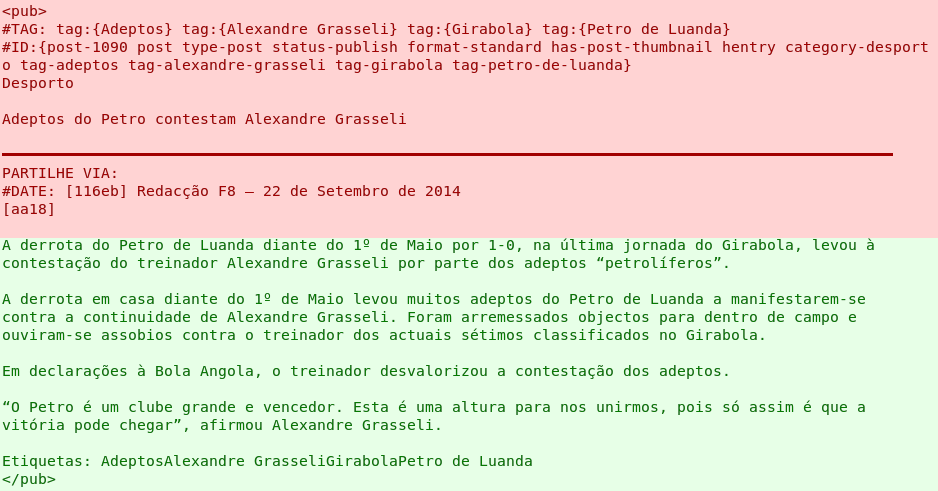
\includegraphics[width=\textwidth]{./example_pub_colored_simple.png}
    \caption{Example Publication}\label{fig:example_pub_simple}
\end{figure}

As can be seen in the example above (Figure~\ref{fig:example_pub_simple}), a
publication is split in roughly 2 parts, the header, in red, where the post's
metadata is stored, and the body or text of the publication, in green. The first
area has tags, id and date which are easy to find due to their
\verb!#NAME{! syntax, but the category and the title (in this example
\textit{``Desporto''} and \textit{``Adpetos de Petro contestam Alexandre
Grasseli''} respectively) have to be parsed using the rest of the header as
context. Next, sometimes there is a sequence delimited by square brackets before
the text, this is also intended to be eliminated.

The third problem to be addressed is the fact that most publications
are repeated throughout the file which can interfere with the counting of the
number of occurrences of each tag.

Lastly, the fourth problem is that \textit{flex} is not unicode aware,
which means that it reads one byte at a time, and since the first byte of the
horizontal bar is the same as the first byte of many other unicode characters,
they are indistinguishable from \textit{flex}'s perspective. To solve this a
simple \textit{bash} script (\texttt{clean\_unicode.sh}) was written to replace
the horizontal bar with a sequence of \verb!#!.

\chapter{Solution}

\section{Parsing contexts}

To parse each publication 4 subcontexts were implemented: \textit{HEADER} (in
red), \textit{DATE} (in blue), \textit{TEXTHEADER} (in yellow) and
\textit{TEXT} (in green) (See Figure~\ref{fig:example_pub_colored}), zones in
white are ignored.

\begin{figure}[h]
    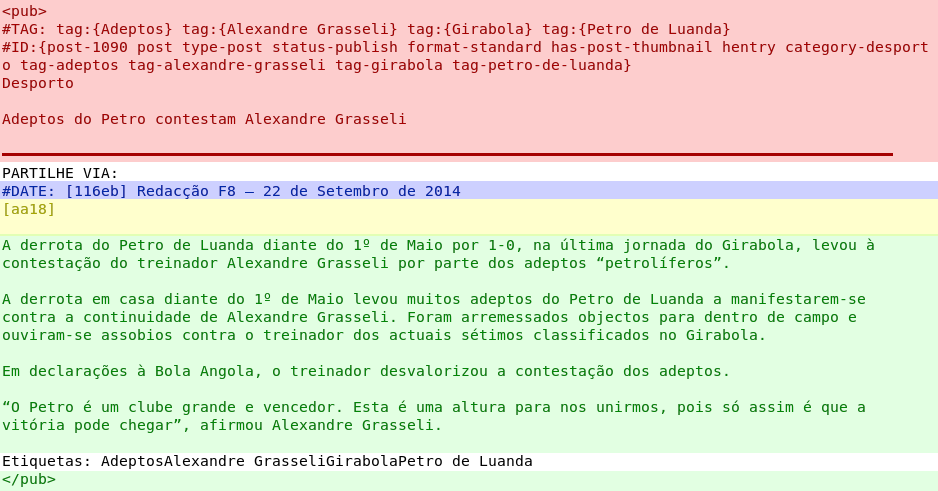
\includegraphics[width=\textwidth]{./example_pub_colored.png}
    \caption{Publication sections breakdown}\label{fig:example_pub_colored}
\end{figure}

\subsection{HEADER}

In the header, the id, tags, category and title are parsed. The tags are
relatively easy to parse, the same goes for the id. To parse the category and
title, a variable is used to check if the category has been parsed, since the
same regular expression is used for both.

\subsection{DATE}

The date context is started when the horizontal bar is found, and all input
strings are ignored until the \texttt{\#DATE} string is matched. At this point
the date is stored and the next context is started.

\subsection{TEXTHEADER}

This context serves only to remove the text between square brackets at the top
of the body, then immediately switches to the \texttt{TEXT} context.

\subsection{TEXT}

This context is very simple, it simply writes what it finds to the output file,
ignoring lines starting with \textit{Etiquetas:} and stopping when it finds the
end of the publication.

\begin{figure}[H]
    %Requires:
%\usepackage{tikz}
%\usetikzlibrary{positioning,automata,decorations.markings}
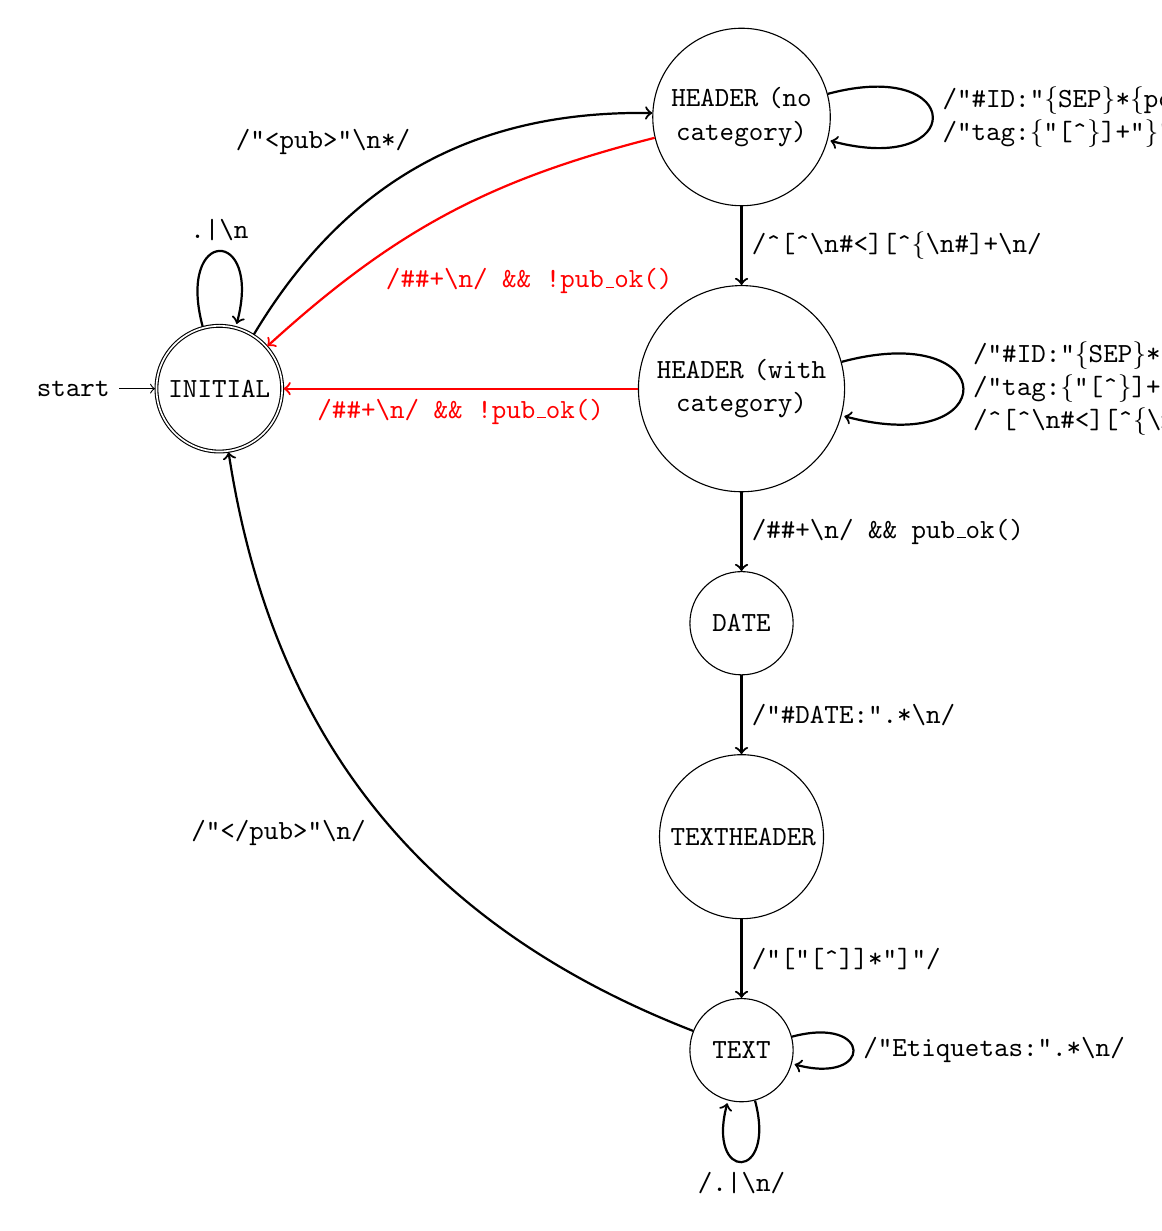
\begin{tikzpicture}[font=\ttfamily,auto]
    \node[state,initial,accepting,text width=13mm,align=center] (initial) {INITIAL};
    \node[state,text width=22mm,align=center] (header1) [right=4.5cm of initial] {HEADER (with category)};
    \node[state,text width=18mm,align=center] (header0) [above=of header1] {HEADER (no category)};
    \node[state,text width=10mm,align=center] (date) [below=of header1] {DATE};
    \node[state,text width=18mm,align=center] (textheader)  [below=of date] {TEXTHEADER};
    \node[state,text width=10mm,align=center] (text) [below=of textheader] {TEXT};
    \path[thick,->]
    (initial)    edge [bend left] node {/"<pub>"\char`\\n*/} (header0)
                 edge [loop above] node {.|\char`\\n} ()

    (header0)    edge [loop right] node [text width=1.5cm,align=center]
                        {/"\#ID:"\{SEP\}*\{post-\{D\}+/
                        /"tag:\{"[\char`\^\}]+"\}"/} ()
                 edge node {/\char`\^[\char`\^\char`\\n\#<][\char`\^\{\char`\\n\#]+\char`\\n/} (header1)
                 edge [bend right=14,red,pos=0.7] node {/\#\#+\char`\\n/ \&\& !pub\_ok()} (initial)

    (header1)    edge [loop right] node [text width=1.5cm,align=center]
                        {/"\#ID:"\{SEP\}*\{post-\{D\}+/
                         /"tag:\{"[\char`\^\}]+"\}"/
                         /\char`\^[\char`\^\char`\\n\#<][\char`\^\{\char`\\n\#]+\char`\\n/
                         } ()
                 edge node {/\#\#+\char`\\n/ \&\& pub\_ok()} (date)
                 edge [red] node {/\#\#+\char`\\n/ \&\& !pub\_ok()} (initial)

    (date)       edge node {/"\#DATE:".*\char`\\n/} (textheader)

    (textheader) edge node {/"["[\char`\^]]*"]"/} (text)

    (text)       edge [loop below] node {/.|\char`\\n/} ()
                 edge [loop right] node {/"Etiquetas:".*\char`\\n/} ()
                 edge [bend left] node {/"</pub>"\char`\\n/} (initial)
    ;
\end{tikzpicture}


    \caption{Parser state machine}\label{fig:parser_state_machine}
\end{figure}

As shown in Figure~\ref{fig:parser_state_machine}, there are two error paths
that can be taken from the \textit{HEADER} context back to the \textit{INITIAL}
context in case the end of the header (marked by the sequence of \verb!#!) is
reached and no `id' has been parsed.

\section{Project Architecture}

Handling of the parsed information is split in two modules,
\texttt{publication} and \texttt{newspaper}.

\subsection{Publication}

This module gathers the information of a single publication to create the
corresponding \texttt{post-id.html} file. When a publication is found this
module is initialized and, as the parser runs, this structure accumulates the
\texttt{id}, \texttt{title}, \texttt{author\_date}, \texttt{category} and
\texttt{tags}. After the header is flushed to its file, every sub
string parsed of the body of the publication is immediately flushed to the file,
as to not accumulate too many bytes in memory.

\subsection{Newspaper}

This module indexes posts and their tags to create several files.
\begin{itemize}
    \item \texttt{index.html}: which references all the parsed posts in
        a list next to their tags;
    \item \texttt{tags.html}: which lists all the tags found next to
        their occurrence count;
    \item \texttt{tagname.hmtl}: for every tag which lists every file with
        that tag.
\end{itemize}

To achieve this, two tables are kept in memory during the parsing of the whole
input string, one associates post ids with the post's title and tags, the other
associates tags with their posts. This way, the relations shown below can be
achieved.

\begin{figure}[H]
    \centering
    \begin{subfigure}{0.54\textwidth}
        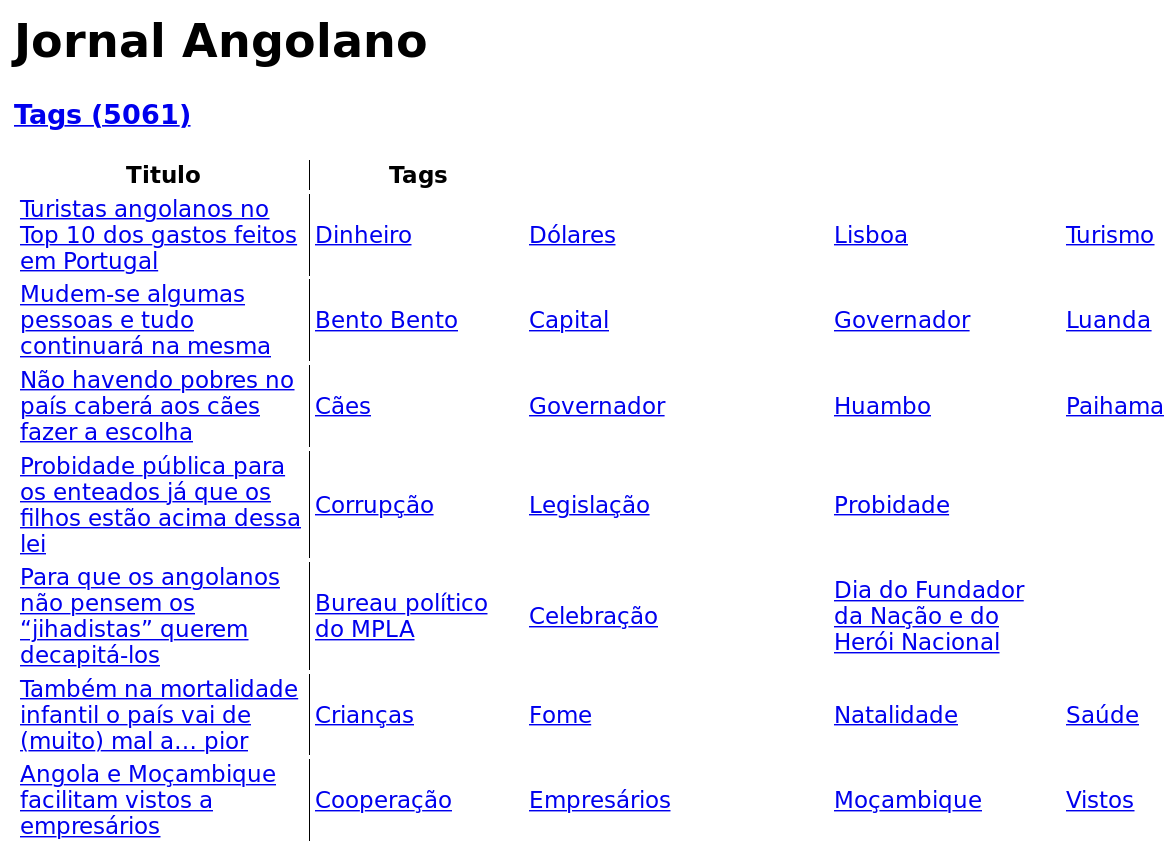
\includegraphics[width=\textwidth]{./index_print.png}
        \caption{index.html}
    \end{subfigure}
    \begin{subfigure}{0.45\textwidth}
        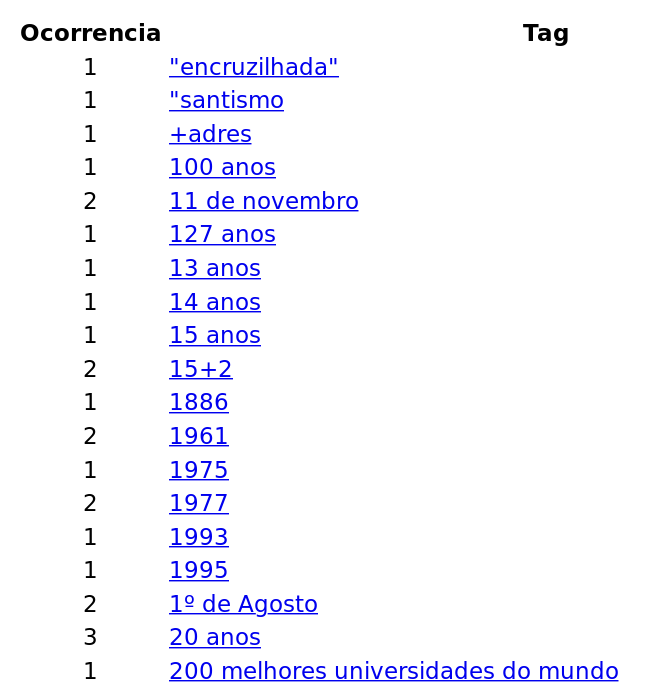
\includegraphics[width=\textwidth]{./tags_print.png}
        \caption{tags.html}
    \end{subfigure}
    \begin{subfigure}{0.45\textwidth}
        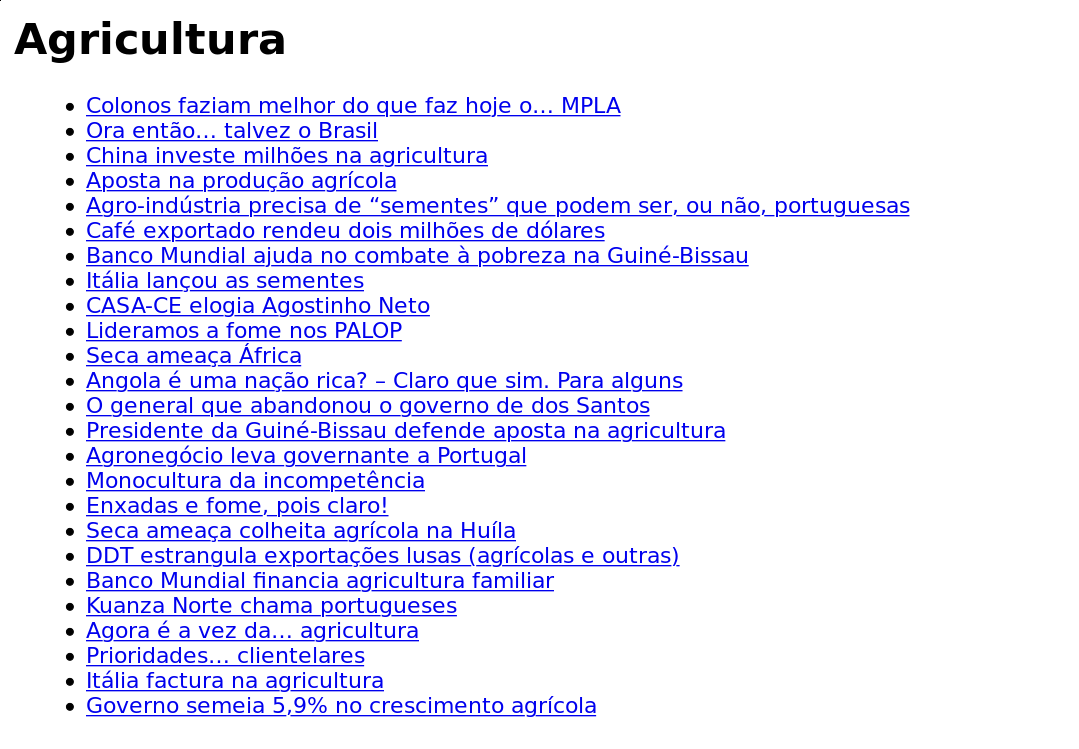
\includegraphics[width=\textwidth]{./tag_print.png}
        \caption{tag.html}
    \end{subfigure}
    \begin{subfigure}{0.54\textwidth}
        
\includegraphics[width=\textwidth]{./publication_print.png}
        \caption{publication.html}
    \end{subfigure}
    \caption{Files generated by the newspaper module}
\end{figure}

\chapter{Performance}

Program performance was a concern during it's implementation. As such, for every
major feature or change made to the program, time and memory benchmarks were
ran. With this system it was possible to detect a huge performance increase
when a simple change of regular expression was made.

One of the regular expressions initially used was incorrect and exceedingly slow.
\begin{figure}[H]
    \centering
    \begin{verbatim}
                        AN   [0-9A-Za-zÀ-ÖØ-öø-ÿ\-]
                        ANS  [0-9A-Za-zÀ-ÖØ-öø-ÿ\- ]

                        <HEADER>{AN}{ANS}+\n
    \end{verbatim}
    \caption{First regular expression to capture the category and title}
\end{figure}

This was made in an effort to capture accented characters, but because, once
again, \textit{flex} is not unicode aware, these ranges did not work properly.
To address this, a different strategy was used: instead of listing what
characters were to be matched, we listed what characters were not to be
matched.

\begin{figure}[H]
    \centering
    \begin{verbatim}
                        <HEADER>^[^\n#<][^{\n#]+\n
    \end{verbatim}
    \caption{Correct regular expression to capture the category and
    title}\label{fig:new-regex}
\end{figure}

This change cut 40\% of the program's runtime, (benchmarked from 2.5s to 1.5s)
because the list of bytes that had to be compared with was smaller, with the
added benefit of capturing more precisely titles that had unicode characters,
such as  ``,  '', --, etc.

The benchmarks made during the software's development can be seen in
Apendix~\ref{app:benches}.

\chapter{Testing}

To test the correctness of the program, a few bash utils were used, notably
common \textit{unix} programs like \textit{grep}, \textit{cat}, \textit{sed},
\textit{sort}, \textit{uniq} and, of course, the \textit{bash}.

\section{Number of articles}

To obtain the number of unique articles in the input file the following command
was used:
\begin{figure}[H]
    \inputminted{bash}{./test_number_of_articles.sh}
    \caption{Count the amount of article repetitions and count the non repeating
    articles.}
\end{figure}

This command outputs the total amount of times articles are repeated, for
example, for the input file tested, the output was the following:

\begin{verbatim}
   3579 2
   1610 1
\end{verbatim}

Meaning that 3579 articles are repeated 2 times and 1610 articles aren't
repeated. Totalling to 5189 articles. To check that the program was producing
the correct amount of articles the command
\verb!ls noticias/post*.html | wc -l! was used.

\section{Counts of given tag}

The next test run was: obtaining the count of individual tags to see if they
match, both in the produced articles, and \texttt{tags.html} file.

To achieve this two commands were used. (As an example the \textit{`regime'}
tag was used).

\begin{figure}[H]
    \inputminted{bash}{./test_count_regime_posts.sh}
    \caption{Count the number of times the `regime' tag comes up in the
    processed articles}
\end{figure}

\begin{figure}[H]
    \inputminted{bash}{./test_count_regime_tags.sh}
    \caption{Show the occurrences of the `regime' tag comes up in the tags.html
    file}
\end{figure}

\section{Count the number of unique tags}

The final test ran was counting the number of unique tags in the input file to
see if it matched the number on the \texttt{index.html} file. To achieve this
the command on figure~\ref{fig:test_count_unique_tags} was used.

\begin{figure}[H]
    \inputminted{bash}{test_count_unique_tags.sh}
    \caption{Count the number of unique tags in the input
    file}\label{fig:test_count_unique_tags}
\end{figure}

\chapter{Conclusion}

In conclusion, all the requirements set out in the assignment were fulfilled, as
well as some extra functionality. The usage of regular expressions to specify
how certain input strings should be handled proved to be very powerful and time
saving.

As an extension of this work a \textit{CSS} file could be added to
improve the visual appeal of the generated pages.

\appendix

\chapter{Flex}

\lstinputlisting[firstline=20,lastline=55,basicstyle=\footnotesize\ttfamily]
{../src/main.l}

\chapter{Benchmarks}\label{app:benches}
\begin{table}[h]
    \begin{tabular}{l c c c c c}
        \multirow{2}{*}{Program Version} & \multirow{2}{*}{mean (s)} &
        \multirow{2}{*}{stddev (s)} & \multicolumn{2}{c}{heap (Mb)} &
        \multirow{2}{*}{stack peak (Kb)}\\

        &    &    & total & peak & \\\toprule

        Not checking for repeated articles
        &2.5803&0.0536&44.220  &0.690  &4.800\\

        Add Article $\to$ Tag Relation
        &2.5413&0.0509&45.390  &1.199  &5.008\\

        Add Index html file
        &2.5771&0.0460&45.672  &1.199  &5.024\\

        Refactor Regex (Figure~\ref{fig:new-regex})
        &1.5959&0.0583&44.674  &1.135  &5.008\\

        Add Tag $\to$ Article Relation
        &2.0040&0.2136&63.731  &1.060  &4.976\\

        Join both Relations
        &1.9717&0.1553&69.157  &1.848  &4.720\\\bottomrule

    \end{tabular}
    \caption{The benchmarks taken during the software's development}
\end{table}

\end{document}

